\documentclass[11pt]{article}
\usepackage{geometry}
\geometry{a4paper, bottom=30mm, top=30mm, left=15mm, right=15mm}
\usepackage{pdfpages}
\usepackage{fancyhdr}
\pagestyle{fancy}
\setlength{\parindent}{0cm}
\setlength{\headheight}{14pt}
\usepackage{tocloft}
\usepackage{parskip}
\usepackage[export]{adjustbox}
\usepackage{float}
\usepackage{subfig}
\usepackage{graphicx}
\graphicspath{{../figures}}
\usepackage{amsmath,blkarray,booktabs,bigstrut, amssymb}
\usepackage{pythonhighlight}
\usepackage{outlines}
\usepackage{soul}
\usepackage[hidelinks]{hyperref}
\usepackage[backend=biber, style=ieee]{biblatex}
\addbibresource{references.bib}
% \bibliographystyle{ieee} % or another style like IEEE, APA, etc.
% \nocite{*}
\usepackage{url}
\setcounter{biburllcpenalty}{7000}
\setcounter{biburlucpenalty}{8000}
\widowpenalty10000
\clubpenalty10000
\setcounter{secnumdepth}{3}
\usepackage[newfloat]{minted}
\usepackage{caption}
\newenvironment{code}{\captionsetup{type=listing}}{}
\SetupFloatingEnvironment{listing}{name=Code Listing}


\begin{document}

\newgeometry{top=20mm}
\begin{titlepage}
    \begin{center}
      \begin{figure}
        
\includegraphics[right]{logo.png}
      \end{figure}
      \vspace*{1cm}
      \textsc{\large ENEL373: Digital Electronics and Devices}\\[0.5cm]
      \textsc{\Large University of Canterbury}\\[3.5cm]
      \linespread{1}
      {\Huge\bfseries This is an Awesome Title \\[0.3cm] for Our First Report} \\
      \vspace*{2cm}
      {\Huge Philip Brand \textit{\Large(15776928)}\\\par}
      {\Huge Michael Brown \textit{\Large(48571923)}\\\par}
      {\Huge Boston Black \textit{\Large(24668421???)}\\\par}
      % ADD YOUR NAME AND STUDENT ID HERE
      \vspace*{3cm}
      {\LARGE \today}
    \end{center}
  \end{titlepage}
\restoregeometry

\fancyhead{}
\fancyhead[L]{\small{ENEL373 - Reaction Timer Project}}
\fancyhead[R]{\small{\today}}

\pagenumbering{roman}

\renewcommand{\baselinestretch}{1.3}\normalsize
\setlength{\cftbeforesecskip}{0.3em}
\renewcommand{\cftsecleader}{\cftdotfill{\cftdotsep}}
\addcontentsline{toc}{section}{Contents}
\tableofcontents\thispagestyle{fancy}
\renewcommand{\baselinestretch}{1}\normalsize

\newpage
\pagenumbering{arabic}

\section{Introduction}
% Outline (in your own words) the project requirements and what you achieved

Human reaction time is the interval between the a stimulus and the response to that stimulus. There are two main types of reaction time; simple, and choice. Simple reaction involves reacting to a singular stimulus, while choice reaction involves choosing the correct response from multiple stimuli. This project aims to implement a simple reaction time recorder on an FPGA in VHDL.

The reaction stimulus test starts with three LEDs that turn off sequentially, with a random delay between each LED turning off. Once the last LED turns off, the user must press a button, and the delay is displayed in milliseconds on 8 7-segment displays. The FPGA stores the reaction delays from the last three trials, and can display the fastest, slowest, and average reaction times. These values can be reset by the user.

\section{Design Summary}
% Summarise your design.

The FPGA reaction stimulus test depends on four major components, those being the 8-digit counter, the ALU, the reaction countdown, and the output select and override. These components are shown in Figure \ref{project_structure}. Each of these components are enabled and disabled via a finite state machine.

% TODO: Add an error state module/mux to the diagram
% TODO: Add better labels to diagram
\begin{figure}[H]
  \centering
  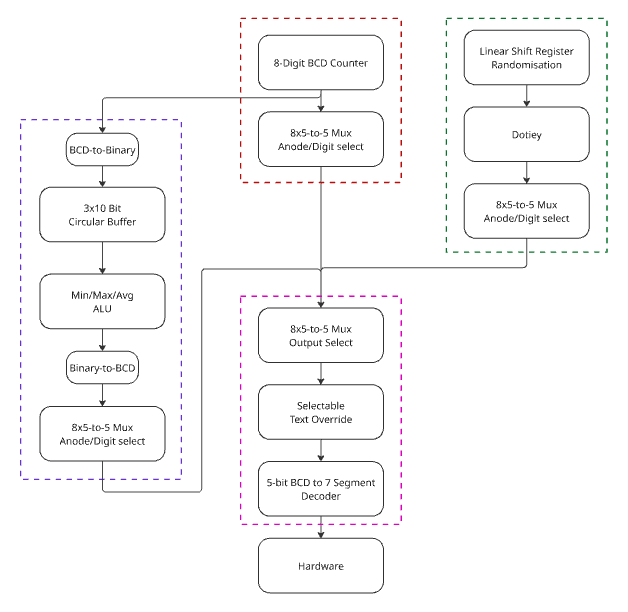
\includegraphics[width=0.7\textwidth]{project_overall_structure.png}
  \caption{Overview of VHDL reaction timer structure}
  \label{project_structure}
\end{figure}

An 8-digit 5-bit-BCD counter is the primary mechanism used to track the reaction time from each stimulus test to the nearest millisecond. Each BCD digit is passed into an 8x5-to-5 mux. The purpose of this mux is to sync the selected output digit with the currently active seven segment display anode, outputting each digit onto its associated display.

% TODO: Review the reference to double dabble here
All the BCD digits from the 8-digit counter are passed directly to ALU module. This module converts the BCD numbers into a 10-bit binary number, then stores the last three reaction times in a circular buffer. This buffer is read by the ALU which calculates the average, minimum, and maximum of the last three reaction times. These times are converted back into BCD using the double dabble algorithm \cite{double_dabble}, and another 8x5-to-5 mux is used to select which digit is output.

A linear shift register is used to provide some randomisation for the countdown sequence at the start of every reaction stimulus test. This time randomisation acts as the trigger for the countdown state, Dotiey, and also has an 8x5-to-5 mux for digit selection.

All three 8x5-to-5 muxes from the three components described above are piped into an 8x5-to-5 mux used for output selection. This mux selects which module to take output from depending on what state is active. The mux output is piped into a text override, which overwrites some of the digits with letters based on state. This is finally piped into a 7 segment decoder, which takes a 5-bit BCD digit and converts it to a 8-bit seven segment display light combination which is piped to hardware.



\section{Expanded Design Summary}
% (~2 pages): Describe the methods your group used to implement your FPGA design. Justify your final design. Support your descriptions and justifications with specific, explicit references to your VHDL source code in the appendix. VHDL descriptions could, for example, include an RTL description. 

\subsection{Design Methods}

The primary focus for the reaction timer project project was to develop VHDL code that is easy to maintain and develop. This led to a heavy focus on modular design and code reuse. Since the project was developed as a group, the other focus was for individual components to be developed and tested by individually, and then put together with minimal issues. 

\subsubsection{Diagramming}

The primary program development method used in this project was to draw program or component flow diagrams before VHDL was written. These digrams detailed the communication between between individual modules, and outlined the overall program structure. Figure \ref{project_structure} shows one such digram outlining each major component in the design and how they're grouped into larger modules. 

Clear communication between group members of the expected inputs and outputs from each component played a significant role in keeping the final assembly simple. Examples include the consistent transfer of characters to be displayed 8x5-to-5 muxes to transmit one character at a time unless otherwise required, such as for the ALU.

\hl{Philip - Michael, do you want to cover some of this?}

\subsubsection{Naming and Syntax Conventions}

Another important aspect of the project ensuring high code quality, readability, and maintainability was strict rules around naming and syntax. This included consistent whitespace, indentation, case, and naming style. For example, all signals within the entity was postfixed with an underscore and whether that signal was an input or output. This can be seen in Listing \ref{code:entity_naming_convention} in Appendix A. This ensured when the components were used in the top-level Behavioural architecture with port mapping, it was easy to see which signals were inputs and outputs.

% TODO: Add capatilisation of signals/input issue

\hl{Add more examples here \dots}
% Could talk about how we tried to have names that described the capabilities of components. eg. 
% timer_8_num_selectable has 8 numbers as output and we can select which one is outputting.
% BCD_8_to_binary has 8 numbers that it converts
% multiiplexer_8_1_4b has 8 inputs, 1 output, and each io is 5 bits (name may need to change)
% counter_3b is a 3 bit counter
% decoder_3b is a 3 bit decoder

% note the consistent _xb at the end descripes how many bits are in the I/O

\subsubsection{Component Reuse}

% Unfinished
In order to reduce the number of components that needed to be created and maintained, components were reused where possible. 

The most versitile example of this was the 8 channel 5 bit mux. The mux took up to 8 5-bit BCD inputs, and selected one of those inputs to be the output. The select lines and number of channels for the mux corresponded the segment display, allowing both to be controlled with the same signal. This capability made it easy to use for displaying timer digits and error message letters. The same mux was also used to select what output to send throught to the display depending on the state. While not all the channels of the mux were used in all usecases. It stil made sense to use the same component as it was proven to work and integrated well with the rest of the system.

\subsubsection{Programming Techniques}

Another method used to implement the FPGA design was pair programming. This had to be done with care, as since the project was done in three-person groups, it would have been easy to leave one person out of the process and result in a lack of their understanding of the code. However, pair programming did help ensure that minimal time was spent debugging, as the observer frequently caught subtleties of VHDL that the programmer missed. Pair programming was used to develop the circular buffer, counters, and FSM.

Since the project the significantly modularised, it was important that individual components could be developed and tested without hindering the development of other components. The method used to achieve this was to use git branching and merging. Individual components were developed on separate branches, tested, and then merged into the main branch. This ensured that the main branch was always stable, and that broken changes could be easily rolled back.

\subsection{Design Justification}
The design of the reaction stimulus test is intended to allow ease of modification or expansion. Keeping modularisation as a high priority during component design allowed each module to view each other module as a ``black box'', interacting only through standardised interfaces. These interfaces were typically a single 5-bit encoded number or letter based on BCD, and were controlled by the generalised 8x5-to-5 mux shown in Appendix \ref{code:8x5_to_5_mux} instead of custom muxes for each output. This further reduced the number of different components required. The only exception to this was the output of all counted BCD digits to the BCD-to-binary convertor as it operated on all digits at once, as shown in Appendix \ref{code:bcd_to_binary}.

A second benefit of each component being a ``black box'' is that as most components interacted only through standardised interfaces, how the components operated behind the scenes was irrelevant. This allowed for significant changes to how a module completed a task without disturbing inter-module communication.

The usage the 8x5-to-5 mux shown in Appendix \ref{code:output_select_mux_instantiation} to select between outputs allows for addition of states as desired by utilizing more mux inputs, with output select lines controlled by the finite state machine. If more states were to be added, then additional muxes can be linked up for more input lines. This shows clear capability for design expansion.

A selectively enabled text override was used to display text in the first two seven-segment displays as it centralised the control of text display. This additionally simplified the other modules as it limited their design to the numeric part of the code.
% TODO: Add justriciation of selectable text override
% TODO: philip sir add justification of lsfr for randon number generation
\newpage

\section{Module Testing}
% A brief section describing how you tested a significant module. Include at least one testbench and associated waveforms that demonstrate the functionality of a module in the report appendix.

% TODO: rename bcd_expanded_out, possibly remove just have a standard 4-bit output
% TODO: reorder waveform to be more logical - put alu output next to operation select and things like that, put clock at the top probably too
% TODO: add testbench waveform for BCD to binary converter

During development of the circular buffer, ALU, and associated data-type converters used to calculate the user reaction time statistics, the output numbers were too small. For example a minimum reaction time of 246 milliseconds would be displayed as 91 milliseconds. Since the delay would be displayed correctly immediate after a test, the problem lay somewhere within the \hl{blue} block in Figure \ref{project_structure}. An assumption was made that the BCD-to-binary converter would be fault-free, since the logic it required was simple. To determine in which module the problem lay, a testbench comprising of the circular buffer, ALU, and binary-to-BCD converter was created. The testbench simulated three write operations to the circular buffer, an ALU operation select, and a trigger for the binary to BCD double-dabble algorithm, followed by reset signal to the circular buffer and binary-to-BCD converter. The testbench stimulus VHDL is in Listing \ref{code:alu_testbench} in \hl{Appendix}.

The major values output by the testbench are the circular buffer contents, the ALU operation select and ALU output, and the binary-to-BCD converted output. These waveforms, as well as the other waveforms such as the clock, circular buffer write, and resets can be seen in Figure \ref{fig:alu_testbench}.

\begin{figure}[H]
  \centering
  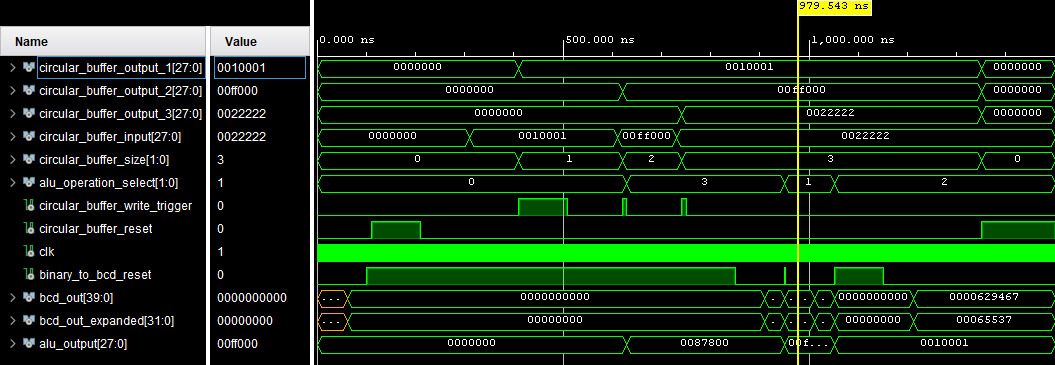
\includegraphics[width=0.99\textwidth]{WhatsApp Image 2025-05-07 at 11.33.07.jpeg}
  \caption{Reaction statistic calculation testbench.}
  \label{fig:alu_testbench}
\end{figure}

The first 750 ns of testbench simulation show the three write operations to the circular buffer. The three circular buffer outputs change exactly as expected, with each write operation setting a new value. The ALU operation select is 3 at 700 ns, and the ALU output is 0087000, which is the correct hexadecimal representation of the average of the three values in the circular buffer. (CHECK THAT). The ALU operation is then set to 1, and the ALU outputs the correct maximum time of 00ff000. The final ALU operation is 2, and the ALU outputs the correct minimum time of 0010001. The binary-to-BCD converter is then triggered, and the BCD output is 00065537, which the correct BCD representation of the 0010001 in hexadecimal.

These waveforms indicated that the problem did not lie where expected, and must have been with the BCD-to-binary converter originally thought of as fault-free. Another testbench was created to test that converter, and, as expected, the converter did not convert correctly. This was rectified by modifying the changing the multiplication factors of 10 from hexadecimal to binary. The fixed testbench waveform can be seen in Appendix something in Figure \ref{fig:correct_converter_tb}.

\newpage

\section{Design \& Implementation Problems}
% Design and/or Implementation problems (can be a separate section or part of the Conclusion): marks for describing problems encountered, and explaining approach to solving them.
% NB: Marks do not depend on whether problems were solved or not, but on the process used.
% 4 marks


\begin{enumerate}
  \item Steven Weddell
  \item Vivado
  \item Vivado
  \item Vivado
  \item VHDL
  \item Steven Weddell
  \item Steven Weddell
  \item Vivado
  \item Vague Error messages
  \item Decimal point issue
  \item Randomisation delay insufficient
  \item Not case sensitive code
  \item Steven Weddell
  \item Vivado
\end{enumerate}

One issue that arose during the development of the seven segment display module which mapped a BCD input to a combination of segments on a display to represent that BCD number was that the provided mappings did not represent the numbers correctly. The solution approach was to first determine whether the BCD input or mapping was incorrect. This was done by tying the BCD input to the green LEDs on the FPGA. This asserted BCD input was correct. To rectify the incorrect mappings, individual segments on a board were tied to the FPGA user switches. Combinations of switches were tested, and when the segments represented a number, the combination of switches was recorded as a mapping.

However, once all the mappings were implemented, we found that our countdown timer failed to display the dots. Alteration of the countdown timer to display temporary digits instead of dots revealed the countdown to be functional. Stepping through the code by hand revealed that, due to the use of the unfamiliar provided seven segment decoder, a line of code was overlooked that overwrote the decimal place value. Disabling this line of code allowed the countdown timer to show dots.

A significantly unexpected issue that appeared during the testing of the finite state machine was deemed as the ``Schrödinger's States'' problem. This originated from the FSM running lines of code designed to change states even while they were commented out. To narrow down the source of the bug, the FSM was reduced to only what was necessary to run a simple reaction timer test without any ALU or error message. From there, states were slowly added back into the FSM and were tied to LEDs that would light up when the new states were activated. This showed additional issues in which an LED would trigger, but the state change wouldn't complete. With the suspicion that a race condition was in play,the issue was fixed by removing the FSM inputs from the sensitivity list of the FSM process, instead tying it to a 10 kHz clock instead. \textcolor{red}{CONFIRM THE CLOCK SPEED}.

There were issues with the simulation software built into the Vivado toolchain. During the design and subsequent simulation of the BCD-to-Binary numeric converter, the Vivado simulator would stop the simulation at the beginning of the numeric conversion, but would not give an error message to indicate an issue. The issue was narrowed down to being a problem with the simulator itself when a bitstream was generated for the whole system so that the convertor could be tested as part of the whole, and no issue was found.

Another issue that arose was regarding case sensitivity in VHDL. Although VHDL is not case sensitive, the constraints file the VHDL interfaces with is. Early on during the project, while developing the clock divider, an error message ``\hl{insert error message here}'' was encountered. The approach to solving this problem was to ask the TAs in the lab what the message meant. However, they were unable to explain the meaning of the message. From there, the clock divider code we wrote was thoroughly compared to the provided clock divider code, and every small difference tested to see if it repaired the error. This determined the issue to be the case of the clock input declared in entity of main module, as lowercase had been used rather than uppercase. This correct case can be seen in Listing \ref{code:entity_naming_convention}.

\newpage

\section{Conclusions}
% Highlight any problems you encountered and how you solved them. Also discuss what you learned and give suggestions on how the project could be improved


\newpage
% There is no need to include a full code listing in your report as your code will be submitted via eng-git. However, reference to a code snippet in an appendix is quite appropriate. Formal citations to books, web articles, open source VHDL code and other sources should be listed in a reference section that uses the IEEE style and format.


\printbibliography

\newpage

\section{Appendix A: Code Listings}

\begin{code}
  \begin{minted}{vhdl}
  
    -- Define module IO
    entity counter_decade is
        Port ( EN_IN : in STD_LOGIC;
               RESET_IN : in STD_LOGIC;
               INCREMENT_IN : in STD_LOGIC;
               COUNT_OUT : out STD_LOGIC_VECTOR (3 downto 0);
               TICK_OUT : out STD_LOGIC);
    end counter_decade;

  \end{minted}
  \captionsetup{belowskip=0pt}
  \captionof{listing}{Entity naming convention example.}
  \label{code:entity_naming_convention}
\end{code}

\vspace*{1cm}

\begin{code}
  \begin{minted}{vhdl}
    library IEEE;
    use IEEE.STD_LOGIC_1164.ALL;
    use IEEE.NUMERIC_STD.ALL;

    entity main is
        Port (  CLK100MHZ : in STD_LOGIC; -- This must be capitalised.
                -- This, and the rest, must be too.
                AN : out STD_LOGIC_VECTOR (7 downto 0) := X"00"; 
                SEVEN_SEG : out STD_LOGIC_VECTOR (7 downto 0) := X"00";
                BTNC : in STD_LOGIC;
                BTNR : in STD_LOGIC;
                BTNL : in STD_LOGIC;
                BTNU : in STD_LOGIC;
                BTND : in STD_LOGIC);  
    end main;
  \end{minted}
  \captionsetup{belowskip=0pt}
  \captionof{listing}{Capitalised port names to avoid errors.}
  \label{code:entity_naming_convention}
\end{code}

\vspace*{1cm}

\begin{code}
  \begin{minted}{vhdl}
    library IEEE;
    use IEEE.STD_LOGIC_1164.ALL;
    
    entity multiplexer_8_1_4b is
        Port ( MUX_IN_0 : in STD_LOGIC_VECTOR (4 downto 0);
               MUX_IN_1 : in STD_LOGIC_VECTOR (4 downto 0);
               MUX_IN_2 : in STD_LOGIC_VECTOR (4 downto 0);
               MUX_IN_3 : in STD_LOGIC_VECTOR (4 downto 0);
               MUX_IN_4 : in STD_LOGIC_VECTOR (4 downto 0);
               MUX_IN_5 : in STD_LOGIC_VECTOR (4 downto 0);
               MUX_IN_6 : in STD_LOGIC_VECTOR (4 downto 0);
               MUX_IN_7 : in STD_LOGIC_VECTOR (4 downto 0);
               SELECT_IN : in STD_LOGIC_VECTOR (2 downto 0);
               MUX_OUT : out STD_LOGIC_VECTOR (4 downto 0));
    end multiplexer_8_1_4b;
    
    architecture Behavioral of multiplexer_8_1_4b is
    begin
        process (SELECT_IN, MUX_IN_0, MUX_IN_1, MUX_IN_2, MUX_IN_3, MUX_IN_4, MUX_IN_5, MUX_IN_6, MUX_IN_7)
        begin
            case(SELECT_IN) is
                when "000" => MUX_OUT <= MUX_IN_0;
                when "001" => MUX_OUT <= MUX_IN_1;
                when "010" => MUX_OUT <= MUX_IN_2;
                when "011" => MUX_OUT <= MUX_IN_3;
                when "100" => MUX_OUT <= MUX_IN_4;
                when "101" => MUX_OUT <= MUX_IN_5;
                when "110" => MUX_OUT <= MUX_IN_6;
                when "111" => MUX_OUT <= MUX_IN_7;
            end case;
        end process;
    end Behavioral;
  \end{minted}
  \captionsetup{belowskip=0pt}
  \captionof{listing}{Generalised 8x5-to-5 mux.}
  \label{code:8x5_to_5_mux}
\end{code}

\vspace*{1cm}

\begin{code}
  \begin{minted}{vhdl}
    entity bcd_8_to_binary is
        Port ( BCD_BUS_IN : in STD_LOGIC_VECTOR (39 downto 0);
              BINARY_OUT : out STD_LOGIC_VECTOR (27 downto 0));
    end bcd_8_to_binary;
  \end{minted}
  \captionsetup{belowskip=0pt}
  \captionof{listing}{BCD to binary converter entity defintion.}
  \label{code:bcd_to_binary}
\end{code}

\vspace*{1cm}

\begin{code}
  \begin{minted}{vhdl}
    ff11: multiplexer_8_1_4b port map (MUX_IN_0 => encoded_reaction_time_digit,
                                       MUX_IN_1 => selected_alu_bcd_digit,
                                       MUX_IN_2 => selected_alu_bcd_digit,
                                       MUX_IN_3 => selected_alu_bcd_digit,
                                       MUX_IN_4 => encoded_error_text,
                                       MUX_IN_5 => encoded_display_placeholder,
                                       MUX_IN_6 => encoded_display_placeholder,
                                       MUX_IN_7 => encoded_dots,
                                       SELECT_IN => encoded_display_input_select,
                                       MUX_OUT => encoded_segment_data);
  \end{minted}
  \captionsetup{belowskip=0pt}
  \captionof{listing}{Component instantiation of output select 8x5-to-5 mux.}
  \label{code:output_select_mux_instantiation}
\end{code}

\vspace*{1cm}
\begin{code}
  \begin{minted}{vhdl}

    simulation_clk : process
    begin
        wait for 1ns;
        clk <= '1';
        wait for 1ns;
        clk <= '0';
    end process;

    simulation : process
    begin
        binary_to_bcd_reset <= '1';
        wait for 10ns;
        circular_buffer_reset <= '1';
        circular_buffer_input <= X"0000000";
        wait for 100ns;
        circular_buffer_reset <= '0';
        wait for 100ns;
        circular_buffer_input <= X"0010001";
        binary_to_bcd_reset <= '1';
        wait for 100ns;
        circular_buffer_write_trigger <= '1';
        wait for 100ns;
        circular_buffer_write_trigger <= '0';
        wait for 100ns;
        circular_buffer_input <= X"00FF000";
        wait for 10ns;
        circular_buffer_write_trigger <= '1';
        wait for 10ns;
        alu_operation_select <= "11";
        circular_buffer_write_trigger <= '0';
        wait for 100ns;
        circular_buffer_input <= X"0022222";
        wait for 10ns;
        circular_buffer_write_trigger <= '1';
        wait for 10ns;
        circular_buffer_write_trigger <= '0';
        wait for 100ns;
        binary_to_bcd_reset <= '0';
        wait for 100ns;
        binary_to_bcd_reset <= '1';
        alu_operation_select <= "01";
        wait for 1ns;
        binary_to_bcd_reset <= '0';
        wait for 100ns;
        binary_to_bcd_reset <= '1';
        alu_operation_select <= "10";
        wait for 100ns;
        binary_to_bcd_reset <= '0';
        wait for 200ns;
        circular_buffer_reset <= '1';
        wait for 100000ns;
    end process;
        

  \end{minted}
  \captionsetup{belowskip=0pt}
  \captionof{listing}{Stimulus for reaction statistic calculation debug testbench.}
  \label{code:alu_testbench}
\end{code}

\end{document}
